\section{Describing hardware devices}

\subsection{Discoverable hardware: USB and PCI}

\begin{frame}{Discoverable hardware}
  \begin{itemize}
  \item Some busses have built-in hardware discoverability mechanisms
  \item Most common busses: USB and PCI
  \item Hardware devices can be enumerated, and their characteristics
    retrieved with just a driver or the bus controller
  \item Useful Linux commands
    \begin{itemize}
    \item \code{lsusb}, lists all USB devices detected
    \item \code{lspci}, lists all PCI devices detected
    \item A detected device does not mean it has a kernel driver
      associated to it!
    \end{itemize}
  \item Association with kernel drivers done based on product
    ID/vendor ID, or some other characteristics of the device: device
    class, device sub-class, etc.
  \end{itemize}
\end{frame}

\subsection{Describing non-discoverable hardware}

\begin{frame}{Describing non-discoverable hardware}
  \begin{columns}
    \column{0.3\textwidth}
    \begin{enumerate}
    \item<1> Directly in the {\bf OS/bootloader code}
    \item<2> Using {\bf ACPI} tables
    \item<3> Using a {\bf Device Tree}
    \end{enumerate}
    \column{0.7\textwidth}
    \only<1> {
      \begin{itemize}
      \item Using compiled data structures, typically in C
      \item How it was done on most embedded platforms in Linux, U-Boot.
      \item Considered not maintainable/sustainable on ARM32, which
        motivated the move to another solution.
      \end{itemize}
    }
    \only<2> {
      \begin{itemize}
      \item On {\em x86} systems, but also on a subset of ARM64 platforms
      \item Tables provided by the firmware
      \end{itemize}
    }
    \only<3> {
      \begin{itemize}
      \item Originates from {\bf OpenFirmware}, defined by Sun, used on
        SPARC and PowerPC
        \begin{itemize}
        \item That's why many Linux/U-Boot functions related to DT have
          a \code{of_} prefix
        \end{itemize}
      \item Now used by most embedded-oriented CPU architectures that run
        Linux: ARC, ARM64, RISC-V, ARM32, PowerPC, Xtensa, MIPS, etc.
      \item Writing/tweaking a DT is necessary when porting Linux to a
        new board, or when connecting additional peripherals
      \end{itemize}
    }
  \end{columns}
\end{frame}

\questionslide{Why is putting description in code not maintainable?}

\begin{frame}{Device Tree: from source to blob}
  \begin{columns}
    \column{0.7\textwidth}
    \begin{itemize}
    \item A tree data structure describing the hardware is written by a
      developer in a {\bf Device Tree Source} file, \code{.dts}
    \item Processed by the {\bf Device Tree Compiler}, \code{dtc}
    \item Produces a more efficient representation: {\bf Device Tree
        Blob}, \code{.dtb}
    \item Additional C preprocessor pass
    \item \code{.dtb} $\rightarrow$ accurately describes the hardware platform in an {\bf OS-agnostic} way.
    \item \code{.dtb} $\approx$ few dozens of kilobytes
    \item DTB also called {\bf FDT}, {\em Flattened Device Tree}, once
      loaded into memory.
      \begin{itemize}
      \item \code{fdt} command in U-Boot
      \item \code{fdt_} APIs
      \end{itemize}
    \end{itemize}
    \column{0.3\textwidth}
    \includegraphics[height=0.7\textheight]{slides/kernel-hw-devices/dts-to-dtb.pdf}
  \end{columns}
\end{frame}

\begin{frame}[fragile]{dtc example}
  \footnotesize
  \begin{columns}[t]
    \column{0.5\textwidth}
    \begin{block}{}
\begin{verbatim}
$ cat foo.dts
/dts-v1/;

/ {
        welcome = <0xBADCAFE>;
        bootlin {
                webinar = "great";
                demo = <1>, <2>, <3>;
        };
};
\end{verbatim}
    \end{block}
    \pause
    \begin{block}{}
\begin{verbatim}
$ dtc -I dts -O dtb -o foo.dtb foo.dts
$ ls -l foo.dt*
-rw-r--r-- 1 thomas thomas 169 ... foo.dtb
-rw-r--r-- 1 thomas thomas 102 ... foo.dts
\end{verbatim}
    \end{block}
    \pause
    \column{0.5\textwidth}
    \begin{block}{}
\begin{verbatim}
$ dtc -I dtb -O dts foo.dtb
/dts-v1/;

/ {
        welcome = <0xbadcafe>;

        bootlin {
                webinar = "great";
                demo = <0x01 0x02 0x03>;
        };
};
\end{verbatim}
    \end{block}
  \end{columns}
\end{frame}

\begin{frame}{Where are Device Tree Sources located?}
  \begin{itemize}
  \item Even though they are OS-agnostic, {\bf no central and
      OS-neutral} place to host Device Tree sources and share them
    between projects
    \begin{itemize}
    \item Often discussed, never done
    \end{itemize}
  \item In practice, the Linux kernel sources can be considered as the
    {\bf canonical location} for Device Tree Source files
    \begin{itemize}
    \item \code{arch/<ARCH>/boot/dts/<vendor>/}
    \item \code{arch/arm/boot/dts} (on ARM 32 architecture before Linux 6.5)
    \item $\approx$ 4500 Device Tree Source files (\code{.dts} and
          \code{.dtsi}) in Linux as of 6.0.
    \end{itemize}
  \item Duplicated/synced in various projects
    \begin{itemize}
    \item U-Boot, Barebox, TF-A
    \end{itemize}
  \end{itemize}
\end{frame}

\begin{frame}{Device Tree base syntax}
  \begin{columns}
    \column{0.5\textwidth}
    \begin{itemize}
    \item Tree of {\bf nodes}
    \item Nodes with {\bf properties}
    \item Node $\approx$ a device or IP block
    \item Properties $\approx$ device characteristics
    \item Notion of {\bf cells} in property values
    \item Notion of {\bf phandle} to point to other nodes
    \item \code{dtc} only does syntax checking, no semantic validation
    \end{itemize}
    \column{0.5\textwidth}
    \begin{center}
      \includegraphics[height=0.6\textheight]{slides/kernel-hw-devices/dt-basic-syntax.pdf}
    \end{center}
  \end{columns}
\end{frame}

\begin{frame}[fragile]{DT overall structure: simplified example}
  \begin{columns}
    \column{0.6\textwidth}
    \begin{onlyenv}<1>
      \begin{block}{}
\begin{minted}[fontsize=\tiny]{perl}
/ {
  #address-cells = <1>;
  #size-cells = <1>;
  model = "TI AM335x BeagleBone Black";
  compatible = "ti,am335x-bone-black", "ti,am335x-bone", "ti,am33xx";

  cpus { ... };
  memory@80000000 { ... };
  chosen { ... };
  ocp {
    intc: interrupt-controller@48200000 { ... };
    usb0: usb@47401300 { ... };
    l4_per: interconnect@44c00000 {
      i2c0: i2c@40012000 { ... };
    };
  };
};
\end{minted}
      \end{block}
    \end{onlyenv}
    \begin{onlyenv}<2>
      \begin{block}{}
\begin{minted}[fontsize=\tiny]{perl}
/ {
  cpus {
    #address-cells = <1>;
    #size-cells = <0>;
    cpu0: cpu@0 {
      compatible = "arm,cortex-a8";
      enable-method = "ti,am3352";
      device_type = "cpu";
      reg = <0>;
    };
  };

  memory@0x80000000 {
    device_type = "memory";
    reg = <0x80000000 0x10000000>; /* 256 MB */
  };

  chosen {
    bootargs = "";
    stdout-path = &uart0;
  };

  ocp { ... };
};
\end{minted}
      \end{block}
    \end{onlyenv}
    \begin{onlyenv}<3>
      \begin{block}{}
\begin{minted}[fontsize=\tiny]{perl}
/ {
  cpus { ... };
  memory@0x80000000 { ... };
  chosen { ... };
  ocp {

    intc: interrupt-controller@48200000 {
      compatible = "ti,am33xx-intc";
      interrupt-controller;
      #interrupt-cells = <1>;
      reg = <0x48200000 0x1000>;
    };

    usb0: usb@47401300 {
      compatible = "ti,musb-am33xx";
      reg = <0x1400 0x400>, <0x1000 0x200>;
      reg-names = "mc", "control";
      interrupts = <18>;
      dr_mode = "otg";
      dmas = <&cppi41dma  0 0 &cppi41dma  1 0 ...>;
      status = "okay";
    };

    l4_per: interconnect@44c00000 {
      i2c0: i2c@40012000 { ... };
    };
  };
};
\end{minted}
      \end{block}
    \end{onlyenv}
    \begin{onlyenv}<4>
      \begin{block}{}
\begin{minted}[fontsize=\tiny]{perl}
/ {
  cpus { ... };
  memory@0x80000000 { ... };
  chosen { ... };

  ocp {
    compatible = "simple-pm-bus";
    clocks = <&l3_clkctrl AM3_L3_L3_MAIN_CLKCTRL 0>;
    clock-names = "fck";
    #address-cells = <1>;
    #size-cells = <1>;

    intc: interrupt-controller@48200000 { ... };
    usb0: usb@47401300 { ... };

    l4_per: interconnect@44c00000 {
      compatible = "ti,am33xx-l4-wkup", "simple-pm-bus";
      reg = <0x44c00000 0x800>, <0x44c00800 0x800>,
            <0x44c01000 0x400>, <0x44c01400 0x400>;
      reg-names = "ap", "la", "ia0", "ia1";
      #address-cells = <1>;
      #size-cells = <1>;

      i2c0: i2c@40012000 { ... };
    };
  };
};
\end{minted}
      \end{block}
    \end{onlyenv}
    \begin{onlyenv}<5>
      \begin{block}{}
\begin{minted}[fontsize=\tiny]{perl}
/ {
  cpus { ... };
  memory@0x80000000 { ... };
  chosen { ... };
  ocp {
    intc: interrupt-controller@48200000 { ... };
    usb0: usb@47401300 { ... };
    l4_per: interconnect@44c00000 {

      i2c0: i2c@40012000 {
        compatible = "ti,omap4-i2c";
        #address-cells = <1>;
        #size-cells = <0>;
        reg = <0x0 0x1000>;
        interrupts = <70>;
        status = "okay";
        pinctrl-names = "default";
        pinctrl-0 = <&i2c0_pins>;
        clock-frequency = <400000>;

        baseboard_eeprom: eeprom@50 {
          compatible = "atmel,24c256";
          reg = <0x50>;
        };
      };
    };
  };
};
\end{minted}
      \end{block}
    \end{onlyenv}
    \column{0.4\textwidth}
    \includegraphics[width=\textwidth]{slides/kernel-hw-devices/simple-hardware.pdf}
  \end{columns}
\end{frame}

\begin{frame}[fragile]{Device Tree inheritance}
  \begin{itemize}
  \item Device Tree files are not monolithic, they can be split in
    several files, including each other.
  \item \code{.dtsi} files are included files, while \code{.dts} files
    are {\em final} Device Trees
    \begin{itemize}
    \item Only \code{.dts} files are accepted as input to \code{dtc}
    \end{itemize}
  \item Typically, \code{.dtsi} will contain
    \begin{itemize}
    \item definitions of SoC-level information
    \item definitions common to several boards
    \end{itemize}
  \item The \code{.dts} file contains the board-level information
  \item The inclusion works by {\bf overlaying} the tree of the
    including file over the tree of the included file, according
    to the order of the \code{#include} directives.
  \item Allows an including file to {\bf override} values specified by
    an included file.
  \item Uses the C pre-processor {\tt \#include} directive
  \end{itemize}
\end{frame}

\begin{frame}{Device Tree inheritance example}
  \begin{center}
    \includegraphics[width=\textwidth]{slides/kernel-hw-devices/dt-inheritance.pdf}
  \end{center}
\end{frame}

\begin{frame}[fragile]{Inheritance and labels}

  \begin{columns}[t]
    \column{0.5\textwidth}
    Doing:
    \begin{block}{soc.dtsi}
      {\tiny
\begin{minted}{perl}
/ {
  ocp {
    uart0: serial@0 {
      compatible = "ti,am3352-uart", "ti,omap3-uart";
      reg = <0x0 0x1000>;
      status = "disabled";
    };
  };
};
\end{minted}
      }
    \end{block}

    \begin{block}{board.dts}
      {\tiny
\begin{minted}{perl}
#include "soc.dtsi"

/ {
  ocp {
    serial@0 {
      status = "okay";
    };
  };
};
\end{minted}
      }
    \end{block}

    \column{0.5\textwidth}
    \begin{onlyenv}<2>
    Is exactly equivalent to:

    \begin{block}{soc.dtsi}
      {\tiny
\begin{minted}{perl}
/ {
  ocp {
    uart0: serial@0 {
      compatible = "ti,am3352-uart", "ti,omap3-uart";
      reg = <0x0 0x1000>;
      status = "disabled";
    };
  };
};
\end{minted}
      }
    \end{block}

    \begin{block}{board.dts}
      {\tiny
\begin{minted}{perl}
#include "soc.dtsi"

&uart0 {
  status = "okay";
};
\end{minted}
        }
      \end{block}

      $\rightarrow$ this solution is now often preferred
      \end{onlyenv}
  \end{columns}

\end{frame}

\begin{frame}{DT inheritance in Bone Black support}
  \begin{center}
    \includegraphics[height=0.8\textheight]{slides/kernel-hw-devices/dt-inheritance-bbb.pdf}
  \end{center}
\end{frame}

\begin{frame}{Device Tree design principles}
  \begin{itemize}
  \item {\bf Describe hardware} (how the hardware is), not
    configuration (how I choose to use the hardware)
  \item {\bf OS-agnostic}
    \begin{itemize}
    \item For a given piece of HW, Device Tree should be the same for
      U-Boot, FreeBSD or Linux
    \item There should be no need to change the Device Tree when updating the OS
    \end{itemize}
  \item Describe {\bf integration of hardware components}, not the internals
    of hardware components
    \begin{itemize}
    \item The details of how a specific device/IP block is working is
      handled by code in device drivers
    \item The Device Tree describes how the device/IP block is
      connected/integrated with the rest of the system: IRQ lines, DMA
      channels, clocks, reset lines, etc.
    \end{itemize}
  \item Like all beautiful design principles, these principles are
    sometimes violated.
  \end{itemize}
\end{frame}

\begin{frame}[fragile]{The properties}
  Device tree properties can:
  \begin{itemize}
  \item Be generic and apply to most nodes
    \begin{itemize}
    \item Their meaning is usually described in one place: the core DT
      schema available at \url{https://github.com/devicetree-org/dt-schema}.
    \item \code{compatible}, \code{reg},
      {\usebeamercolor[fg]{code}\path{#address-cells}}, etc
    \end{itemize}
  \item Cover common consumer-provider relationships
    \begin{itemize}
    \item Their meaning is either described in the
      \href{https://github.com/devicetree-org/dt-schema}{dt-schema}
      GitHub repository or under \kfile{Documentation/devicetree/bindings}.
    \item \code{clocks}, \code{interrupts}, \code{regulators}, etc
    \end{itemize}
  \item Subsystem specific
    \begin{itemize}
    \item All devices of a certain class may use them, often starting
      with the class name
    \item \code{spi-cpha}, \code{i2c-scl-internal-delay-ns}, \code{nand-ecc-engine},
      \code{mac-address}, etc
    \end{itemize}
  \item Vendor/device specific
    \begin{itemize}
    \item To describe uncommon or very specific properties
    \item Always described in the device's binding file and prefixed with \code{<vendor>,}
    \item \code{ti,hwmods}, \code{xlnx,num-channels}, \code{nxp,tx-output-mode}, etc
    \end{itemize}
  \item Some of them are deprecated, watch out the bindings!
  \end{itemize}
\end{frame}

\begin{frame}{The {\tt compatible} property}
  \begin{itemize}
  \item Is a list of strings
    \begin{itemize}
    \item From the most specific to the least specific
    \end{itemize}
  \item Describes the specific {\bf binding} to which the node complies.
  \item It uniquely identifies the {\bf programming model} of the
    device.
  \item Practically speaking, it is used by the operating system to
    find the {\bf appropriate driver} for this device.
  \item When describing real hardware, the typical form is
    \code{vendor,model}
  \item Examples:
    \begin{itemize}
    \item \code{compatible = "arm,armv7-timer";}
    \item \code{compatible = "st,stm32mp1-dwmac", "snps,dwmac-4.20a";}
    \item \code{compatible = "regulator-fixed";}
    \item \code{compatible = "gpio-keys";}
    \end{itemize}
  \item Special value: \code{simple-bus} $\rightarrow$ bus where all
    sub-nodes are memory-mapped devices
  \end{itemize}
\end{frame}

\begin{frame}{{\tt compatible} property and Linux kernel drivers}
  \begin{columns}
    \column{0.6\textwidth}
    \begin{itemize}
    \item Linux identifies as {\bf platform devices}:
      \begin{itemize}
      \item Top-level DT nodes with a \code{compatible} string
      \item Sub-nodes of \code{simple-bus}
        \begin{itemize}
        \item Instantiated automatically at boot time
        \end{itemize}
      \end{itemize}
    \item Sub-nodes of I2C controllers $\rightarrow$ {\em I2C devices}
    \item Sub-nodes of SPI controllers $\rightarrow$ {\em SPI devices}
    \item Each Linux driver has a table of compatible strings it supports
      \begin{itemize}
      \item \kstruct{of_device_id}\code{[]}
      \end{itemize}
    \item When a DT node compatible string matches a given driver, the
      device is {\em bound} to that driver.
    \end{itemize}
    \column{0.4\textwidth}
    \includegraphics[width=\textwidth]{slides/kernel-hw-devices/dt-to-devices.pdf}
  \end{columns}
\end{frame}

\begin{frame}[fragile]{Matching with drivers in Linux: platform driver}
  \begin{block}{\kfile{drivers/i2c/busses/i2c-omap.c}}
    {\tiny
\begin{minted}{c}
static const struct of_device_id omap_i2c_of_match[] = {
        {
                .compatible = "ti,omap4-i2c",
                .data = &omap4_pdata,
        },
        {
                .compatible = "ti,omap3-i2c",
                .data = &omap3_pdata,
        },
        [...]
        { },
};
MODULE_DEVICE_TABLE(of, omap_i2c_of_match);

[...]

static struct platform_driver omap_i2c_driver = {
        .probe          = omap_i2c_probe,
        .remove         = omap_i2c_remove,
        .driver         = {
                .name   = "omap_i2c",
                .pm     = &omap_i2c_pm_ops,
                .of_match_table = of_match_ptr(omap_i2c_of_match),
        },
};
\end{minted}
    }
  \end{block}
\end{frame}

\begin{frame}[fragile]{Matching with drivers in Linux: I2C driver}
  \begin{block}{\kfile{sound/soc/codecs/cs42l51.c}}
    {\tiny
\begin{minted}{c}
const struct of_device_id cs42l51_of_match[] = {
        { .compatible = "cirrus,cs42l51", },
        { }
};
MODULE_DEVICE_TABLE(of, cs42l51_of_match);
\end{minted}
    }
  \end{block}
  \begin{block}{\kfile{sound/soc/codecs/cs42l51-i2c.c}}
    {\tiny
\begin{minted}{c}
static struct i2c_driver cs42l51_i2c_driver = {
        .driver = {
                .name = "cs42l51",
                .of_match_table = cs42l51_of_match,
                .pm = &cs42l51_pm_ops,
        },
        .probe = cs42l51_i2c_probe,
        .remove = cs42l51_i2c_remove,
        .id_table = cs42l51_i2c_id,
};
\end{minted}
    }
  \end{block}
\end{frame}

\begin{frame}[fragile]{{\tt reg} property}
  \begin{itemize}
  \item Most important property after \code{compatible}
  \item {\bf Memory-mapped} devices: base physical address and size of
    the memory-mapped registers. Can have several entries for multiple
    register areas.
\begin{onlyenv}<1>
\begin{block}{}
\begin{verbatim}
sai4: sai@50027000 {
    reg = <0x50027000 0x4>, <0x500273f0 0x10>;
};
\end{verbatim}
\end{block}
\end{onlyenv}
\pause
  \item {\bf I2C} devices: address of the device on the I2C bus.
\begin{onlyenv}<2>
\begin{block}{}
\begin{verbatim}
&i2c1 {
   hdmi-transmitter@39 {
      reg = <0x39>;
   };
   cs42l51: cs42l51@4a {
      reg = <0x4a>;
   };
};
\end{verbatim}
\end{block}
\end{onlyenv}
\pause
  \item {\bf SPI} devices: chip select number
\begin{onlyenv}<3>
\begin{block}{}
\begin{verbatim}
&qspi {
        flash0: mx66l51235l@0 {
                reg = <0>;
        };
        flash1: mx66l51235l@1 {
                reg = <1>;
        };
};
\end{verbatim}
\end{block}
\end{onlyenv}
\pause
\item The unit address must be the address of the first \code{reg}
  entry.
\begin{onlyenv}<4>
\begin{block}{}
\begin{verbatim}
sai4: sai@50027000 {
    reg = <0x50027000 0x4>, <0x500273f0 0x10>;
};
\end{verbatim}
\end{block}
\end{onlyenv}
  \end{itemize}
\end{frame}

\begin{frame}[fragile]{{\tt cells} property}
  \begin{itemize}
  \item Property numbers shall fit into 32-bit containers called
    \code{cells}
  \item The compiler does not maintain information about the number of
    entries, the OS just receives 4 independent \code{cells}
    \begin{itemize}
      \begin{onlyenv}<1>
      \item Example with a \code{reg} property using 2 entries of 2 cells:
        \begin{block}{}
\begin{verbatim}
    reg = <0x50027000 0x4>, <0x500273f0 0x10>;
\end{verbatim}
        \end{block}
      \item The OS cannot make the difference with:
        \begin{block}{}
\begin{verbatim}
    reg = <0x50027000>, <0x4>, <0x500273f0>, <0x10>;
    reg = <0x50027000 0x4 0x500273f0>, <0x10>;
    reg = <0x50027000>, <0x4 0x500273f0 0x10>;
    reg = <0x50027000 0x4 0x500273f0 0x10>;
\end{verbatim}
        \end{block}
      \end{onlyenv}
    \end{itemize}
    \pause
  \item Need for other properties to declare the right formatting:
    \begin{itemize}
    \item {\tt \#address-cells}: Indicates the number of cells
      used to carry the address
    \item {\tt \#size-cells}: Indicates the number of cells
      used to carry the size of the range
    \end{itemize}
  \item The parent-node declares the children \code{reg} property
    formatting
    \begin{itemize}
    \item Platform devices need memory ranges
      \begin{onlyenv}<2>
        \begin{block}{}
\begin{verbatim}
module@a0000 {
    #address-cells = <1>;
    #size-cells = <1>;

    serial@1000 {
        reg = <0x1000 0x10>, <0x2000 0x10>;
    };
};
\end{verbatim}
        \end{block}
      \end{onlyenv}
      \pause
    \item SPI devices need chip-selects
      \begin{onlyenv}<3>
        \begin{block}{}
\begin{verbatim}
spi@300000 {
    #address-cells = <1>;
    #size-cells = <0>;

    flash@1 {
        reg = <1>;
    };
};
\end{verbatim}
        \end{block}
      \end{onlyenv}
    \end{itemize}
  \end{itemize}
\end{frame}

\begin{frame}{Status property}
  \begin{itemize}
  \item The \code{status} property indicates if the device is really in
    use or not
    \begin{itemize}
    \item \code{okay} or \code{ok} $\rightarrow$ the device is really
      in use
    \item any other value, by convention \code{disabled} $\rightarrow$
      the device is not in use
    \end{itemize}
  \item In Linux, controls if a device is instantiated
  \item In \code{.dtsi} files describing SoCs: all devices that
    interface to the outside world have \code{status = "disabled";}
  \item Enabled on a per-device basis in the board \code{.dts}
  \end{itemize}
\end{frame}

\begin{frame}[fragile]{Resources: interrupts, clocks, DMA, reset lines, ...}
  \begin{columns}
  \column{0.5\textwidth}
  \begin{itemize}
  \item Common pattern for resources shared by multiple hardware
    blocks
    \begin{itemize}
    \item Interrupt lines
    \item Clock controllers
    \item DMA controllers
    \item Reset controllers
    \item ...
    \end{itemize}
  \item A Device Tree node describing the {\em controller} as a device
  \item References from other nodes that use resources provided by
    this {\em controller}
  \end{itemize}
  \column{0.5\textwidth}
\begin{block}{}
{\tiny
\begin{minted}{perl}
intc: interrupt-controller@a0021000 {
   compatible = "arm,cortex-a7-gic";
   #interrupt-cells = <3>;
   interrupt-controller;
   reg = <0xa0021000 0x1000>, <0xa0022000 0x2000>;
};

rcc: rcc@50000000 {
   compatible = "st,stm32mp1-rcc", "syscon";
   reg = <0x50000000 0x1000>;
   #clock-cells = <1>;
   #reset-cells = <1>;
};

dmamux1: dma-router@48002000 {
   compatible = "st,stm32h7-dmamux";
   reg = <0x48002000 0x1c>;
   #dma-cells = <3>;
   clocks = <&rcc DMAMUX>;
   resets = <&rcc DMAMUX_R>;
};

spi3: spi@4000c000 {
   interrupts = <GIC_SPI 51 IRQ_TYPE_LEVEL_HIGH>;
   clocks = <&rcc SPI3_K>;
   resets = <&rcc SPI3_R>;
   dmas = <&dmamux1 61 0x400 0x05>,  <&dmamux1 62 0x400 0x05>;
};
\end{minted}
}
\end{block}
\end{columns}
\end{frame}

\begin{frame}[fragile]{Generic suffixes}
  \begin{itemize}
  \item \code{xxx-gpios}
    \begin{itemize}
    \item When drivers need access to GPIOs
    \item May be subsystem-specific or vendor-specific
    \item Examples: \code{enable-gpios}, \code{cts-gpios}, \code{rts-gpios}
    \end{itemize}
  \item \code{xxx-names}
    \begin{itemize}
    \item Sometimes naming items is relevant
    \item Allows drivers to perform lookups by name rather than ID
    \item The order of definition of each item still matters
    \item Examples: \code{gpio-names}, \code{clock-names},
      \code{reset-names}
    \end{itemize}
  \end{itemize}
  \begin{block}{}
    \begin{minted}{perl}
uart0@4000c000 {
    dmas = <&edma 26 0>, <&edma 27 0>;
    dma-names = "tx", "rx";
    ...
};
    \end{minted}
  \end{block}
\end{frame}

\begin{frame}{How to validate Device Tree content? 1/2}
  \begin{itemize}
  \item \code{compatible} properties enforce a specific programming model
  \item OS expect a specific set of properties in each node
    \begin{itemize}
    \item The syntax is fixed
    \item The content is defined (number of items, their size, their meaning)
    \item Some properties are mandatory
    \end{itemize}
  \item How do I check the validity of a DT snippet?
    \begin{itemize}
    \item How do I avoid losing half a day on a typo?
    \item Looking at drivers to understand the DT structure tends to make it OS-specific
    \end{itemize}
  \end{itemize}
\end{frame}

\begin{frame}[fragile]{How to validate Device Tree content? 2/2}
  \begin{columns}
    \column{0.7\textwidth}
    \begin{itemize}
    \item {\bf Device Tree Specifications} $\rightarrow$ base Device
      Tree syntax + number of standard properties.
      \begin{itemize}
      \item \url{https://www.devicetree.org/specifications/}
      \item Not sufficient to describe the wide variety of hardware.
      \end{itemize}
    \item {\bf Device Tree Bindings} $\rightarrow$ describes how a piece
      of HW should be described
      \begin{itemize}
      \item Common bindings are defined in an external repository
        \url{https://github.com/devicetree-org/dt-schema/tree/main/dtschema/schemas}
        \begin{itemize}
        \item Generic properties: \code{reg} or
          {\usebeamercolor[fg]{code}\path{#address-cells}}
        \item Consumer bindings: \code{interrupts}, \code{clocks},
          \code{dmas}, etc
        \end{itemize}
      \item Device-specific descriptions are in the Linux kernel sources
        \kdir{Documentation/devicetree/bindings}
      \end{itemize}
    \end{itemize}
    \column{0.3\textwidth}
    \includegraphics[width=\textwidth]{slides/kernel-hw-devices/dt-spec.png}
  \end{columns}
\end{frame}

\begin{frame}{Device Tree bindings}
  \begin{itemize}
      \item Bindings are improved as part of the Linux kernel
        contribution process
      \item They are carefully reviewed by DT binding maintainers and
        can only be merged once approved by them
      \item Need for automated verifications:
        \begin{itemize}
        \item Legacy: human readable .txt documents, hardly parsable
          by tools
        \item Current norm: YAML-written specifications, easy to parse
          by humans and tools at the same time!
        \end{itemize}
    \end{itemize}
\end{frame}

\begin{frame}[fragile]{Device Tree binding: legacy style}
  \begin{columns}[t]
    \column{0.55\textwidth}
    \begin{block}{\kfileversion{Documentation/devicetree/bindings/i2c/i2c-omap.txt}{5.13.19}}
      \begin{minted}[fontsize=\tiny]{text}
I2C for OMAP platforms

-Required properties :
- compatible : Must be
       "ti,omap2420-i2c" for OMAP2420 SoCs
       "ti,omap2430-i2c" for OMAP2430 SoCs
       "ti,omap3-i2c" for OMAP3 SoCs
       "ti,omap4-i2c" for OMAP4+ SoCs
       "ti,am654-i2c", "ti,omap4-i2c" for AM654 SoCs
       "ti,j721e-i2c", "ti,omap4-i2c" for J721E SoCs
       "ti,am64-i2c", "ti,omap4-i2c" for AM64 SoCs
- ti,hwmods : Must be "i2c<n>", n being the instance number (1-based)
- #address-cells = <1>;
- #size-cells = <0>;

Recommended properties :
- clock-frequency : Desired I2C bus clock frequency in Hz. Otherwise
  the default 100 kHz frequency will be used.

Optional properties:
- Child nodes conforming to i2c bus binding
    \end{minted}
    \end{block}
    \column{0.45\textwidth}
    \begin{block}{}
      \begin{minted}[fontsize=\tiny]{text}
Note: Current implementation will fetch base address, irq
and dma from omap hwmod data base during device registration.
Future plan is to migrate hwmod data base contents into
device tree blob so that, all the required data will be used
from device tree dts file.

Examples :

i2c1: i2c@0 {
    compatible = "ti,omap3-i2c";
    #address-cells = <1>;
    #size-cells = <0>;
    ti,hwmods = "i2c1";
    clock-frequency = <400000>;
};
      \end{minted}
    \end{block}
  \end{columns}

\end{frame}

\begin{frame}[fragile]{Device Tree binding: YAML style}
  \kfile{Documentation/devicetree/bindings/i2c/ti,omap4-i2c.yaml}
  \begin{columns}[t]
    \column{0.33\textwidth}
    \begin{block}{}
      {\fontsize{5}{6}\selectfont
\begin{minted}{yaml}
# SPDX-License-Identifier: (GPL-2.0-only OR BSD-2-Clause)
%YAML 1.2
---
$id: http://devicetree.org/schemas/i2c/ti,omap4-i2c.yaml#
$schema: http://devicetree.org/meta-schemas/core.yaml#

title: I2C controllers on TI's OMAP and K3 SoCs

maintainers:
  - Vignesh Raghavendra <vigneshr@ti.com>

properties:
  compatible:
    oneOf:
      - enum:
          - ti,omap2420-i2c
          - ti,omap2430-i2c
          - ti,omap3-i2c
          - ti,omap4-i2c
      - items:
          - enum:
              - ti,am4372-i2c
              - ti,am64-i2c
              - ti,am654-i2c
              - ti,j721e-i2c
          - const: ti,omap4-i2c

  reg:
    maxItems: 1
\end{minted}
      }
    \end{block}
    \column{0.33\textwidth}
    \begin{block}{}
      {\fontsize{5}{6}\selectfont
\begin{minted}{yaml}
  interrupts:
    maxItems: 1

  clocks:
    maxItems: 1

  clock-names:
    const: fck

  clock-frequency: true

  power-domains: true

  "#address-cells":
    const: 1

  "#size-cells":
    const: 0

  ti,hwmods:
    description:
      Must be "i2c<n>", n being [...]
    $ref: /schemas/types.yaml#/definitions/string
    deprecated: true

required:
  - compatible
  - reg
  - interrupts
\end{minted}
      }
    \end{block}
    \column{0.33\textwidth}
    \begin{block}{}
      {\fontsize{5}{6}\selectfont
\begin{minted}{yaml}
additionalProperties: false

if:
  properties:
    compatible:
      enum:
        - ti,omap2420-i2c
        - ti,omap2430-i2c
        - ti,omap3-i2c
        - ti,omap4-i2c
then:
  properties:
    ti,hwmods:
      items:
        - pattern: "^i2c([1-9])$"
else:
  properties:
    ti,hwmods: false

examples:
  - |
    #include <dt-bindings/interrupt-controller/irq.h>
    #include <dt-bindings/interrupt-controller/arm-gic.h>

    main_i2c0: i2c@2000000 {
        compatible = "ti,j721e-i2c", "ti,omap4-i2c";
        reg = <0x2000000 0x100>;
        interrupts = <GIC_SPI 200 IRQ_TYPE_LEVEL_HIGH>;
    };
\end{minted}
      }
    \end{block}
  \end{columns}
\end{frame}

\begin{frame}{Validating Device Trees}
  \begin{itemize}
  \item \code{dtc} only does syntactic validation
  \item YAML bindings allow to do semantic validation
  \item Linux kernel \code{make} rules:
    \begin{itemize}
    \item \code{make dt_binding_check}\\
      verify that YAML bindings are valid, particularly useful if you
      write examples!
    \item \code{make dtbs_check}\\
      validate DTs currently enabled against YAML bindings
    \end{itemize}
  \item The combination of DTS and bindings growing, it may sometimes be
    relevant to only check against a subset of matching schema by adding
    the \code{DT_SCHEMA_FILES} specifier on the \code{make} command line:
    \begin{itemize}
    \item eg. \code{make
        DT_SCHEMA_FILES=Documentation/devicetree/bindings/trivial-devices.yaml
      dtbs_check}\\
    \item Can be used with both \code{dt_binding_check} and \code{dtbs_check}
    \end{itemize}
  \end{itemize}
\end{frame}

\begin{frame}[fragile]{Bindings syntax: base structure}
  \begin{columns}
    \column{0.4\textwidth}
    \begin{block}{}
      {\fontsize{5}{6}\selectfont
\begin{minted}{yaml}
# SPDX-License-Identifier: (GPL-2.0-only OR BSD-2-Clause)
%YAML 1.2
---
$id: http://devicetree.org/schemas/<path>/<file-name.yaml>#
$schema: http://devicetree.org/meta-schemas/core.yaml#

title: <Type and name of the device>

maintainers:
  - John Doe <john@doe.com>

description: |
  Some multiline text.

  At an additional indentation level.

# This line is a comment
properties:
  prop-a:
    ...

  prop-b:
    ...
\end{minted}
      }
    \end{block}
    \column{0.6\textwidth}
    Each YAML file defines one DT hierarchical level (up to two when there
    are children nodes expected)
    \begin{itemize}
    \item {\usebeamercolor[fg]{code}\path{%YAML}} defines the expected
      language version
    \item \code{$id} maybe not a real URL, but a unique identifier
    \item \code{$schema} refers to the base meta-schema this file should
      be validated against (in the Github repository mentioned
      previously)
    \item \code{properties:} where the definitions start
    \item All possible properties should be listed
      \begin{itemize}
      \item dash-separated lowercase names
      \item names followed by a colon '\code{:}' and a new line
      \end{itemize}
    \item Every indentation level is 2 spaces
    \item An empty line between property definitions
    \end{itemize}
  \end{columns}
\end{frame}

\begin{frame}[fragile]{Bindings syntax: types}
  \begin{columns}
    \column{0.4\textwidth}
    \begin{block}{}
      {\fontsize{5}{6}\selectfont
\begin{minted}{yaml}
properties:
  # A boolean property, basically a yes or no
  pin-x-not-wired:      # pin-x-not-wired;
    type: boolean

  # Expects a single 32-bit numerical value
  start-offset:         # start-offset: <0x1000>;
    $ref: /schemas/types.yaml#/definitions/uint32

  # The suffix already enforces a numerical value!
  # In this case if there is no additional constraint
  # we set the property to 'true'
  my-freq-hz: true      # my-freq-hz = <100000>;

  # Expects an array of 32-bit numerical values
  supported-rates:      # supported-rates = <25>, <50>;
    $ref: /schemas/types.yaml#/definitions/uint32-array

  # A string value is expected
  instruction-set:      # instruction-set = "extended";
    $ref: /schemas/types.yaml#/definitions/string

  # Phandles will be expected
  sampling-lines:       # sampling-lines = <&pioA 1>, <&pioA 5>;
    $ref: /schemas/types.yaml#/definitions/phandle-array

  # Here as well, but no need to repeat the constraint
  # because '-gpios' is a generic suffix
  reset-gpios: true     # reset-gpios = <&gpio SOC_SPEC_IDX>;
\end{minted}
      }
    \end{block}
    \column{0.6\textwidth}
    \begin{itemize}
    \item Properties must be typed, either with the \code{type:} or the
      \code{ref:} keyword.
      \begin{itemize}
      \item Boolean properties require no value
      \item Numerical values can be signed or unsigned but should always
        be 32-bit wide
      \item Strings should always be fully defined (see next slides)
      \item Arrays and matrices are possible as well
      \end{itemize}
    \item Generic bindings already set the type for many properties:
      \begin{itemize}
      \item Their values/items numbers can be constrained further
      \item The types don't need to be repeated however
      \end{itemize}
    \item \code{dt-schema} will enforce a type based on the property
      name suffix, eg: \code{-hz}, \code{-ohms}, \code{-us}
    \end{itemize}
  \end{columns}
\end{frame}

\begin{frame}[fragile]{Bindings syntax: child nodes}
  \begin{columns}
    \column{0.4\textwidth}
    \begin{block}{}
      {\fontsize{5}{6}\selectfont
\begin{minted}{yaml}
properties:
  # The sub-node can only be named: child-node
  child-node:
    type: object

patternProperties:
  # The sub-node name is flexible, eg: child@1000, child@2a, etc
  "^child@[a-f0-9]+$":
    type: object
\end{minted}
      }
    \end{block}
    \column{0.6\textwidth}
    \begin{itemize}
    \item From a yaml-schema perspective, children nodes are just another
      property
    \item A specific type shall however be enforced:
      \begin{itemize}
      \item \code{type: object}
      \end{itemize}
    \item Under the main \code{properties} keyword, property/sub-node
      names are fixed
      \begin{itemize}
      \item If the sub-node name is dynamic, we shall define it under
        another top-level keyword, \code{patternProperties} and use
        pattern-matching regexes for the naming
      \end{itemize}
    \end{itemize}
  \end{columns}
\end{frame}

\begin{frame}{Bindings syntax: expressing constraints}
  Besides defining precisely the different properties and their type,
  the content of the property values must also be constrained.
  \begin{itemize}
  \item All properties can get an additional \code{description}
    parameter, which is only readable by humans
  \item We try to maximize the constraints to minimize human errors
  \item One new line per constraint
  \end{itemize}
\end{frame}

\begin{frame}[fragile]{Bindings syntax: numerical constraints}
  \begin{columns}
    \column{0.4\textwidth}
    \begin{block}{}
      {\fontsize{5}{6}\selectfont
\begin{minted}{yaml}
properties:
  # The numerical value is bounded
  # This is valid:
  # frequency-hz = <100000>;
  # frequency-hz = <0x40000>; /* 262144 Hz */
  # This is not:
  # frequency-hz = <0>;
  # frequency-hz = <&gpio 10>;
  frequency-hz:
    minimum: 10000
    maximum: 400000
    default: 100000

  # This is an array with either 1 or 2 members
  # This is valid:
  # cs-gpios = <&gpioA 1>;
  # cs-gpios = <&gpioA 1>, <gpioA 5>;
  # This is not:
  # cs-gpios = <&gpioA 1>, <gpioA 5>, <gpioA 6>;
  # cs-gpios = <50>;
  cs-gpios:
    minItems: 1
    maxItems: 2
\end{minted}
      }
    \end{block}
    \column{0.6\textwidth}
    \begin{itemize}
    \item Example of constraints:
      \begin{itemize}
      \item \code{minimum:}/\code{maximum:} min/max values for a
        single value
      \item \code{default:} for a default value
      \item \code{minItems:}/\code{maxItems:} min/max number of
        items in an array
      \end{itemize}
    \end{itemize}
  \end{columns}
\end{frame}

\begin{frame}[fragile]{Bindings syntax: lists and dictionaries}
  \begin{columns}
    \column{0.4\textwidth}
    \begin{block}{}
      {\fontsize{5}{6}\selectfont
\begin{minted}{yaml}
properties:
  # This is a very common compatible definition
  # The only allowed combinations are (order matters):
  # compatible = "vendor1,compat", "generic,compat";
  # compatible = "vendor2,compat", "generic,compat";
  # compatible = "legacy-compat";
  compatible:
    oneOf:
      - items:
          - enum:
              - vendor1,compat
              - vendor2,compat
          - const: generic,compat
      - items:
          - const: legacy-compat

  # Property name is known by dt-schema, type will be inferred
  # No need for minItems/maxItems, 2 will be implied from
  # the main items list!
  clocks:
    items:
      - description: Interconnect
      - description: External bus

  # This is valid:   strength = <0>, <5>;
  # This is invalid: strength = <0>;
  #                  strength = <0>, <8>;
  strength:
    $ref: /schemas/types.yaml#/definitions/uint32-array
    minItems: 2
    maxItems: 2
    items:
      maximum: 5
\end{minted}
      }
    \end{block}
    \column{0.6\textwidth}
    \begin{itemize}
    \item Expressing several possible property values\\
      (works with numbers and strings):
      \begin{itemize}
      \item Force a single expected value: \code{const}
      \item Allow taking one value from a list: \code{enum}
        \begin{itemize}
        \item watch out the indentation: 2 spaces from the previous
          keyword and a dash
        \end{itemize}
      \end{itemize}
    \item \code{const}/\code{enum} can be grouped within an \code{items}
      list, where each \code{items} sub-entry must be observed
    \item We can build abstract conditional lists (eg. on top of
      \code{items} rather than proper values like with
      \code{const}/\code{enum}:
      \begin{itemize}
      \item XOR using \code{oneOf}
      \item OR using \code{anyOf}
      \item AND using \code{allOf}
      \end{itemize}
    \end{itemize}
  \end{columns}
\end{frame}

\begin{frame}[fragile]{Bindings syntax: referencing other bindings}
  \begin{columns}
    \column{0.4\textwidth}
    \begin{block}{}
      {\fontsize{5}{6}\selectfont
\begin{minted}{yaml}
# All properties/constraints defined in generic-controller.yaml
# will apply (but they can be tuned/overwritten below)
allOf:
  - $ref: generic-controller.yaml

properties:
  # Tune a property defined in generic-controller.yaml
  prop-a:
    maximum: 1

  # Allow a new, more specific property
  vendor,specific-prop: true

  # common-child-constraints.yaml will enforce a base set of
  # properties and rules
  child-node:
    type: object
    $ref: common-child-constraints.yaml
\end{minted}
      }
    \end{block}
    \column{0.6\textwidth}
    \begin{itemize}
    \item It is possible to write "common" constraints in a YAML file
      and refer to it
      \begin{itemize}
      \item Very usual when describing a certain type of controller
        \begin{itemize}
        \item Refer to the generic constraints with a top-level
          \code{allOf}
        \item Add constraints which are specific to the hardware
          implementation
        \end{itemize}
      \item Possible to constrain children nodes by referencing another
        YAML file
      \end{itemize}
    \end{itemize}
  \end{columns}
\end{frame}

\begin{frame}[fragile]{Bindings syntax: altering on presence of properties}
  \begin{columns}
    \column{0.4\textwidth}
    \begin{block}{}
      {\fontsize{5}{6}\selectfont
\begin{minted}{yaml}
properties:
  compatible:
    enum:
      - compat1
      - compat2

  prop-a: true

  prop-b: true

  prop-c: true

dependencies:
  prop-a: [ 'prop-b' ]
  prop-b: [ 'prop-a' ]

allOf:
  - if:
      properties:
        compatible:
          contains:
            const: compat1
    then:
      properties:
        prop-c: false
\end{minted}
      }
    \end{block}
    \column{0.6\textwidth}
    \begin{itemize}
    \item Sometimes more dynamic descriptions are needed
      \begin{itemize}
      \item Dependencies between properties
        \begin{itemize}
        \item A property may be needed if there is another property
        \item If both or none shall be present, the dependency should be
          expressed twice (in both directions)
        \end{itemize}
      \item Changing constraints based on a property
        \begin{itemize}
        \item Can be expressed using \code{if}/\code{else} statements
          under the top-level \code{allOf}
        \item Typical case: a \code{compatible} implies tweaking a
          constraint
        \end{itemize}
      \end{itemize}
    \end{itemize}
  \end{columns}
\end{frame}

\begin{frame}[fragile]{Bindings syntax: enforcing correct properties only}
  \begin{columns}
    \column{0.4\textwidth}
    \begin{block}{}
      {\fontsize{5}{6}\selectfont
\begin{minted}{yaml}
allOf:
  - $ref: generic-file.yaml

properties:
  prop-a: true

  prop-b: true

  child-node:
    type: object
    properties:
      prop-c: true
      prop-d: true

    required:
      - prop-c

    # No additional property than the ones above
    # will be allowed inside child-node
    additionalProperties: false

required:
  - prop-a

# Only properties defined below or coming from
# generic-file.yaml will be allowed
unevaluatedProperties: false
\end{minted}
      }
    \end{block}
    \column{0.6\textwidth}
    \begin{itemize}
    \item YAML files list properties and add constraints to them
      \begin{itemize}
      \item It is still possible to add undefined properties
      \item It is still possible to forget defining a mandatory
        property
      \end{itemize}
    \item We need further constraints to spot typos and unexpected
      properties
      \begin{itemize}
      \item \code{required} forces the presence
      \item \code{additionalProperties} prevents any property not
        defined in {\bf this} file to be used
      \item \code{unevaluatedProperties} prevents any property not
        defined in this file nor referenced (through
        \code{allOf} or {\usebeamercolor[fg]{code}\path{$ref}}) to be
        used
      \end{itemize}
    \end{itemize}
  \end{columns}
\end{frame}

\begin{frame}[fragile]{Bindings syntax: validating your own bindings}
  \begin{columns}
    \column{0.4\textwidth}
    \begin{block}{}
      {\fontsize{5}{6}\selectfont
\begin{minted}{yaml}
properties:
  prop-a: true
  prop-b: true

  child-node:
    type: object
    additionalProperties: false

required:
  - prop-a

unevaluatedProperties: false

example:
  - |
    node@1000 {
      prop-a;
    };
\end{minted}
      }
    \end{block}
    \column{0.6\textwidth}
    \begin{itemize}
    \item It is very recommended to test your bindings before testing
      your DTS
      \begin{itemize}
      \item Add \code{examples} at the end of your file!
      \item Examples are indented with 4 spaces
      \end{itemize}
    \end{itemize}
  \end{columns}
\end{frame}

\begin{frame}
  \frametitle{References}
  \begin{columns}
    \column{0.6\textwidth}
       \begin{itemize}
       \item Device Tree 101 webinar, Thomas Petazzoni (2021):\\
	     Slides: \url{https://bootlin.com/blog/device-tree-101-webinar-slides-and-videos/}\\
	     Video: \url{https://youtu.be/a9CZ1Uk3OYQ}
       \item Kernel documentation
         \begin{itemize}
         \item \kdochtmldir{driver-api/driver-model}
         \item \kdochtmldir{devicetree}
         \item \kdochtml{filesystems/sysfs}
         \end{itemize}
      \item \url{https://devicetree.org}
       \item The kernel source code
         \begin{itemize}
         \item Full of examples of other drivers!
         \item Reference DT binding implementation:
           \kfile{Documentation/devicetree/bindings/example-schema.yaml}
         \end{itemize}
       \end{itemize}
    \column{0.4\textwidth}
    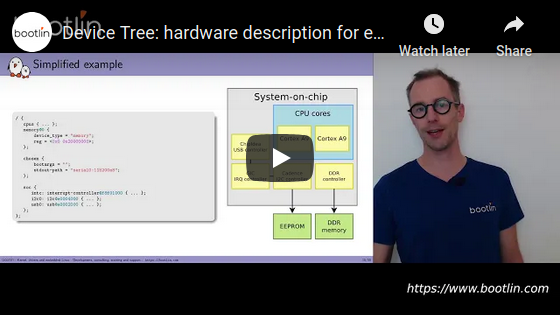
\includegraphics[width=\textwidth]{common/device-tree-video.jpg}
  \end{columns}
\end{frame}

\setuplabframe
{Describing hardware devices}
{
  \begin{itemize}
  \item Browse and update Device Trees.
  \item Use GPIO LEDs.
  \item Modify the Device Tree to enable an I2C controller and describe
    an I2C device.
  \item Write a yaml binding to validate a device description.

  \end{itemize}
}
